%% LyX 2.3.7 created this file.  For more info, see http://www.lyx.org/.
%% Do not edit unless you really know what you are doing.
\documentclass[journal,article,submit,pdftex,moreauthors]{Definitions/mdpi}
\usepackage[utf8]{inputenc}
\usepackage{array}
\usepackage{float}
\usepackage{booktabs}
\usepackage{url}
\usepackage{graphicx}

\makeatletter

%%%%%%%%%%%%%%%%%%%%%%%%%%%%%% LyX specific LaTeX commands.

\Title{EEGO: an extended version of Eel and grouper optimizer for global
optimization problems}

\TitleCitation{EEGO: an extended version of Eel and grouper optimizer for global
optimization problems}

\Author{Glykeria Kyrou$^{1}$, Vasileios Charilogis$^{2}$ and Ioannis G.
Tsoulos$^{3,*}$}

\AuthorNames{Glykeria Kyrou, Vasileios Charilogis and Ioannis G. Tsoulos }

\AuthorCitation{Kyrou, G.; Charilogis, V.; Tsoulos, I.G. }


\address{$^{1}$\quad{}Department of Informatics and Telecommunications,
University of Ioannina, 47150 Kostaki Artas, Greece; g.kyrou@uoi.gr\\
$^{2}$\quad{}Department of Informatics and Telecommunications, University
of Ioannina, 47150 Kostaki Artas, Greece; v.charilog@uoi.gr\\
$^{3}\quad$Department of Informatics and Telecommunications, University
of Ioannina, 47150 Kostaki Artas, Greece;itsoulos@uoi.gr}


\corres{Correspondence: itsoulos@uoi.gr}


\abstract{The problems of finding a global minimum of a function are increasingly
applied to real-world problems. As a result, a variety of computational
techniques have been developed to locate the global minimum with some
certainty. A decisive role is played by evolutionary techniques, which
simulate natural processes and aim to find the global minimum of multidimensional
functions. A recently introduced evolutionary technique is the optimal
Eel and Grouper (EGO) algorithm, which is inspired by the symbiotic
interaction and foraging strategy of eels and groupers in marine ecosystems.
The EGO algorithm is characterized by its reliability in locating
the global minimum. In this paper, modifications are proposed that
aim to improve the reliability and speed of the above technique, such
as the application of a termination technique based on stochastic
observations and an innovative sampling method. The proposed method
was tested on several problems from the relevant literature and a
comparative study was made with other global optimization techniques
with promising results.}


\keyword{Global optimization, Meta-heuristics, Stochastic techniques, Evolutionary
methods, Swarm based methods.s}

\newcommand*\LyXZeroWidthSpace{\hspace{0pt}}
\DeclareTextSymbolDefault{\textquotedbl}{T1}
%% Because html converters don't know tabularnewline
\providecommand{\tabularnewline}{\\}

%%%%%%%%%%%%%%%%%%%%%%%%%%%%%% User specified LaTeX commands.
%  LaTeX support: latex@mdpi.com 
%  For support, please attach all files needed for compiling as well as the log file, and specify your operating system, LaTeX version, and LaTeX editor.

%=================================================================


% For posting an early version of this manuscript as a preprint, you may use "preprints" as the journal and change "submit" to "accept". The document class line would be, e.g., \documentclass[preprints,article,accept,moreauthors,pdftex]{mdpi}. This is especially recommended for submission to arXiv, where line numbers should be removed before posting. For preprints.org, the editorial staff will make this change immediately prior to posting.

%--------------------
% Class Options:
%--------------------
%----------
% journal
%----------
% Choose between the following MDPI journals:
% acoustics, actuators, addictions, admsci, adolescents, aerospace, agriculture, agriengineering, agronomy, ai, algorithms, allergies, alloys, analytica, animals, antibiotics, antibodies, antioxidants, applbiosci, appliedchem, appliedmath, applmech, applmicrobiol, applnano, applsci, aquacj, architecture, arts, asc, asi, astronomy, atmosphere, atoms, audiolres, automation, axioms, bacteria, batteries, bdcc, behavsci, beverages, biochem, bioengineering, biologics, biology, biomass, biomechanics, biomed, biomedicines, biomedinformatics, biomimetics, biomolecules, biophysica, biosensors, biotech, birds, bloods, blsf, brainsci, breath, buildings, businesses, cancers, carbon, cardiogenetics, catalysts, cells, ceramics, challenges, chemengineering, chemistry, chemosensors, chemproc, children, chips, cimb, civileng, cleantechnol, climate, clinpract, clockssleep, cmd, coasts, coatings, colloids, colorants, commodities, compounds, computation, computers, condensedmatter, conservation, constrmater, cosmetics, covid, crops, cryptography, crystals, csmf, ctn, curroncol, currophthalmol, cyber, dairy, data, dentistry, dermato, dermatopathology, designs, diabetology, diagnostics, dietetics, digital, disabilities, diseases, diversity, dna, drones, dynamics, earth, ebj, ecologies, econometrics, economies, education, ejihpe, electricity, electrochem, electronicmat, electronics, encyclopedia, endocrines, energies, eng, engproc, ent, entomology, entropy, environments, environsciproc, epidemiologia, epigenomes, est, fermentation, fibers, fintech, fire, fishes, fluids, foods, forecasting, forensicsci, forests, foundations, fractalfract, fuels, futureinternet, futureparasites, futurepharmacol, futurephys, futuretransp, galaxies, games, gases, gastroent, gastrointestdisord, gels, genealogy, genes, geographies, geohazards, geomatics, geosciences, geotechnics, geriatrics, hazardousmatters, healthcare, hearts, hemato, heritage, highthroughput, histories, horticulturae, humanities, humans, hydrobiology, hydrogen, hydrology, hygiene, idr, ijerph, ijfs, ijgi, ijms, ijns, ijtm, ijtpp, immuno, informatics, information, infrastructures, inorganics, insects, instruments, inventions, iot, j, jal, jcdd, jcm, jcp, jcs, jdb, jeta, jfb, jfmk, jimaging, jintelligence, jlpea, jmmp, jmp, jmse, jne, jnt, jof, joitmc, jor, journalmedia, jox, jpm, jrfm, jsan, jtaer, jzbg, kidney, kidneydial, knowledge, land, languages, laws, life, liquids, literature, livers, logics, logistics, lubricants, lymphatics, machines, macromol, magnetism, magnetochemistry, make, marinedrugs, materials, materproc, mathematics, mca, measurements, medicina, medicines, medsci, membranes, merits, metabolites, metals, meteorology, methane, metrology, micro, microarrays, microbiolres, micromachines, microorganisms, microplastics, minerals, mining, modelling, molbank, molecules, mps, msf, mti, muscles, nanoenergyadv, nanomanufacturing, nanomaterials, ncrna, network, neuroglia, neurolint, neurosci, nitrogen, notspecified, nri, nursrep, nutraceuticals, nutrients, obesities, oceans, ohbm, onco, oncopathology, optics, oral, organics, organoids, osteology, oxygen, parasites, parasitologia, particles, pathogens, pathophysiology, pediatrrep, pharmaceuticals, pharmaceutics, pharmacoepidemiology, pharmacy, philosophies, photochem, photonics, phycology, physchem, physics, physiologia, plants, plasma, pollutants, polymers, polysaccharides, poultry, powders, preprints, proceedings, processes, prosthesis, proteomes, psf, psych, psychiatryint, psychoactives, publications, quantumrep, quaternary, qubs, radiation, reactions, recycling, regeneration, religions, remotesensing, reports, reprodmed, resources, rheumato, risks, robotics, ruminants, safety, sci, scipharm, seeds, sensors, separations, sexes, signals, sinusitis, skins, smartcities, sna, societies, socsci, software, soilsystems, solar, solids, sports, standards, stats, stresses, surfaces, surgeries, suschem, sustainability, symmetry, synbio, systems, taxonomy, technologies, telecom, test, textiles, thalassrep, thermo, tomography, tourismhosp, toxics, toxins, transplantology, transportation, traumacare, traumas, tropicalmed, universe, urbansci, uro, vaccines, vehicles, venereology, vetsci, vibration, viruses, vision, waste, water, wem, wevj, wind, women, world, youth, zoonoticdis 

%---------
% article
%---------
% The default type of manuscript is "article", but can be replaced by: 
% abstract, addendum, article, book, bookreview, briefreport, casereport, comment, commentary, communication, conferenceproceedings, correction, conferencereport, entry, expressionofconcern, extendedabstract, datadescriptor, editorial, essay, erratum, hypothesis, interestingimage, obituary, opinion, projectreport, reply, retraction, review, perspective, protocol, shortnote, studyprotocol, systematicreview, supfile, technicalnote, viewpoint, guidelines, registeredreport, tutorial
% supfile = supplementary materials

%----------
% submit
%----------
% The class option "submit" will be changed to "accept" by the Editorial Office when the paper is accepted. This will only make changes to the frontpage (e.g., the logo of the journal will get visible), the headings, and the copyright information. Also, line numbering will be removed. Journal info and pagination for accepted papers will also be assigned by the Editorial Office.

%------------------
% moreauthors
%------------------
% If there is only one author the class option oneauthor should be used. Otherwise use the class option moreauthors.

%---------
% pdftex
%---------
% The option pdftex is for use with pdfLaTeX. If eps figures are used, remove the option pdftex and use LaTeX and dvi2pdf.

%=================================================================
% MDPI internal commands - do not modify
\firstpage{1} 
 
\setcounter{page}{\@firstpage} 

\pubvolume{1}
\issuenum{1}
\articlenumber{0}
\pubyear{2024}
\copyrightyear{2024}
%\externaleditor{Academic Editor: Firstname Lastname} % For journal Automation, please change Academic Editor to "Communicated by"
\datereceived{}
\daterevised{ } % Comment out if no revised date
\dateaccepted{}
\datepublished{}
%\datecorrected{} % Corrected papers include a "Corrected: XXX" date in the original paper.
%\dateretracted{} % Corrected papers include a "Retracted: XXX" date in the original paper.
\hreflink{https://doi.org/} % If needed use \linebreak
%\doinum{}
%------------------------------------------------------------------
% The following line should be uncommented if the LaTeX file is uploaded to arXiv.org
%\pdfoutput=1

%=================================================================
% Add packages and commands here. The following packages are loaded in our class file: fontenc, inputenc, calc, indentfirst, fancyhdr, graphicx, epstopdf, lastpage, ifthen, lineno, float, amsmath, setspace, enumitem, mathpazo, booktabs, titlesec, etoolbox, tabto, xcolor, soul, multirow, microtype, tikz, totcount, changepage, attrib, upgreek, cleveref, amsthm, hyphenat, natbib, hyperref, footmisc, url, geometry, newfloat, caption

%=================================================================
%% Please use the following mathematics environments: Theorem, Lemma, Corollary, Proposition, Characterization, Property, Problem, Example, ExamplesandDefinitions, Hypothesis, Remark, Definition, Notation, Assumption
%% For proofs, please use the proof environment (the amsthm package is loaded by the MDPI class).

%=================================================================
% The fields PACS, MSC, and JEL may be left empty or commented out if not applicable
%\PACS{J0101}
%\MSC{}
%\JEL{}

%%%%%%%%%%%%%%%%%%%%%%%%%%%%%%%%%%%%%%%%%%
% Only for the journal Diversity
%\LSID{\url{http://}}

%%%%%%%%%%%%%%%%%%%%%%%%%%%%%%%%%%%%%%%%%%
% Only for the journal Applied Sciences:
%\featuredapplication{Authors are encouraged to provide a concise description of the specific application or a potential application of the work. This section is not mandatory.}
%%%%%%%%%%%%%%%%%%%%%%%%%%%%%%%%%%%%%%%%%%

%%%%%%%%%%%%%%%%%%%%%%%%%%%%%%%%%%%%%%%%%%
% Only for the journal Data:
%\dataset{DOI number or link to the deposited data set in cases where the data set is published or set to be published separately. If the data set is submitted and will be published as a supplement to this paper in the journal Data, this field will be filled by the editors of the journal. In this case, please make sure to submit the data set as a supplement when entering your manuscript into our manuscript editorial system.}

%\datasetlicense{license under which the data set is made available (CC0, CC-BY, CC-BY-SA, CC-BY-NC, etc.)}

%%%%%%%%%%%%%%%%%%%%%%%%%%%%%%%%%%%%%%%%%%
% Only for the journal Toxins
%\keycontribution{The breakthroughs or highlights of the manuscript. Authors can write one or two sentences to describe the most important part of the paper.}

%%%%%%%%%%%%%%%%%%%%%%%%%%%%%%%%%%%%%%%%%%
% Only for the journal Encyclopedia
%\encyclopediadef{Instead of the abstract}
%\entrylink{The Link to this entry published on the encyclopedia platform.}
%%%%%%%%%%%%%%%%%%%%%%%%%%%%%%%%%%%%%%%%%%

%%%%%%%%%%%%%%%%%%%%%%%%%%%%%%%%%%%%%%%%%%
% Only for the journal Advances in Respiratory Medicine
%\addhighlights{yes}
%\renewcommand{\addhighlights}{%

%\noindent This is an obligatory section in “Advances in Respiratory Medicine”, whose goal is to increase the discoverability and readability of the article via search engines and other scholars. Highlights should not be a copy of the abstract, but a simple text allowing the reader to quickly and simplified find out what the article is about and what can be cited from it. Each of these parts should be devoted up to 2~bullet points.\vspace{3pt}\\
%\textbf{What are the main findings?}
% \begin{itemize}[labelsep=2.5mm,topsep=-3pt]
% \item First bullet.
% \item Second bullet.
% \end{itemize}\vspace{3pt}
%\textbf{What is the implication of the main finding?}
% \begin{itemize}[labelsep=2.5mm,topsep=-3pt]
% \item First bullet.
% \item Second bullet.
% \end{itemize}
%}
%%%%%%%%%%%%%%%%%%%%%%%%%%%%%%%%%%%%%%%%%%

\makeatother

\begin{document}
\maketitle

\section{Introduction}

The basic goal of global optimization is to find the global minimum
by searching for the appropriate scope of the underlying objective
problem. Primarily, a global optimization method aims to discover
the global minimum of a continuous multidimensional function, and
it is defined as
\begin{equation}
x^{*}=\mbox{arg}\min_{x\in S}f(x)\label{eq:eq1}
\end{equation}
with $S$: 
\[
S=\left[a_{1},b_{1}\right]\times\left[a_{2},b_{2}\right]\times\ldots\left[a_{n},b_{n}\right]
\]

During the past years many researchers have published systematic reviews
on global optimization \citep{plhroforikh,computer,computer1}. Furthermore,
global optimization has appeared in many practical problems from real
world, such as mathematics \citep{maths,maths-1,maths2,key-maths3},
physics \citep{fusikh,fusikh1,fysikhh}, chemistry \citep{xhmeia,xhmeia1,xhmeia2}
and medicine \citep{iatrikh,iatrikh1,medicine}. Optimization methods
are divided into two categories, deterministic \citep{determistic,determistic1,determistic2}
and stochastic \citep{stohastic,stohastic1,stohastic2}.\textbf{ }In
the first category, there are techniques aimed at identifying the
total minimum with some certainty, such as interval methods \citep{key-1,interval2}
and are usually distinguished by their complex implementation. The
vast majority of global optimization algorithms belong to \LyXZeroWidthSpace\LyXZeroWidthSpace stochastic
methods that have simpler implementation and can also be applied to
large -scale problems. Among the stochastic techniques one finds a
large group of methods that have been explored intensively in recent
years, the so - called Swarm Intelligence algorithms.

Swarm intelligence algorithms \citep{swarm1,swarm2,swarm} are inspired
by the collective behavior of insects and other animals. These algorithms
mimic systems in which agents interact locally and cooperate worldwide
to solve optimization problems. Swarm intelligence algorithms are
very important tools for dealing with complex optimization problems
in a wide range of applications \citep{APPS}. Some examples of these
methods are the Whale Optimization Algorithm (WOA) algorithm \citealp{WOA,WOA1,WOA2},
the Sine Cosine algorithm (SCA) algorithm \citep{SCA,SCA1,SCA2,sca1},
the Salp Swarm algorithm (SSA) algorithm \citep{ssaa,SSA,SSA1,SSA2}
etc. These methods simulate a series of complex interactions between
biological species \citep{search algorithm,several metaheuristic algorithms },
such as:
\begin{enumerate}
\item Naturalism: Where two species can live in an ecosystem without affecting
each other. 
\item Predation, where one creature dies by feeding another. 
\item Parasitism: where one species causes harm to another without always
killing it. 
\item In competitive mode, the same or different organizations compete for
resources. 
\item Mutualism \citep{mutualism-parasitism,mutualistic,Competition in mutualistic systems}:
when two organisms have a beneficial interaction. 
\end{enumerate}
Among swarm intelligence algorithms one can find the Eel and Grouper
(EGO) algorithm, which is inspired by the symbiotic interaction and
foraging strategy of eels and groupers in marine ecosystems.\textbf{
}Bshary et al. \citep{hunting between groupers and giant moray eels in the Red Sea}
consider that target ingestion, something observed in eels and groupers,
is a necessary condition for interspecific cooperative hunting to
occur. Intraspecific predation could increase the hunting efficiency
of predators by mammals. According to Ali Mohammadzadeh and Seyedali
Mirjalili the EGO optimization algorithm \citep{Eel and grouper optimizer}
generates a set of random answers, then stores the best answers found
so far, allocates them to the target point, and changes the answers
with them. As the number of iterations increases, the limits of the
sine function are changed to enhance the phase of finding the best
solution. This method stops the process when the iteration exceeds
the maximum number. Because the EGO optimization algorithm generates
and boosts a collection of random responses, it has the advantage
of increased local optimum discovery and avoidance compared to individual
methods.

This paper introduces some modifications to the EGO algorithm in order
to improve its efficiency. The proposed amendments are presented below:
\begin{itemize}
\item The addition of a sampling technique based on the K-means method \citep{kmeans2,kmeans-ereunhtikh-koinothta}.
The sampled points will help to find the global minimum of the function
in the most efficient way. Additionally, by using this method, points
that are in proximity can be rejected.
\item The use of a termination technique based on stochastic observations.
At each iteration of the algorithm, the smallest value is recorded.
Once it remains stable for a predetermined number of iterations, the
method terminates. The present termination method helps with the fastest
termination without unnecessarily wasting computing time.
\item Application of randomness in the definition of the range of the positions
of candidate solutions.
\end{itemize}
The rest of this paper is divided into the following sections: in
section \ref{sec:Materials-and-Methods}, the proposed method is fully
described, in section \ref{sec:Results} the experimental results
and statistical comparisons are outlined and finally in section \ref{sec:Conclusions}
some conclusions and guidelines for future improvements are discussed.

\section{The proposed method\label{sec:Materials-and-Methods}}

The main steps of the base EGO algorithm and the proposed modifications
are described in detail in this section.

\subsection{The main steps of the algorithm}

The main steps of the used global optimization method are the following:
\begin{enumerate}
\item \textbf{Initialization step}.
\begin{enumerate}
\item \textbf{Define} as $N_{c}$ the number of elements in the search Agents
\item \textbf{Define} as $N_{g}$, the maximum number of allowed iterations.
\item \textbf{Initialize} randomly the search agents $x_{i},\ i=1,\ldots,N_{c}$
in set $S$. 
\item \textbf{Set} $t=0$, the iteration counter.
\item \textbf{Set} $s_{r}=0$, the starvation rate of the algorithm. 
\item \textbf{Set} $m=1$, this parameter influences how the variables $f_{1},f_{2}$
are defined, which in turn affects the calculation of new positions.
When $m=1$, it introduces randomness to the range of positions before
the update, while in the inactive state, the range remains fixed.
\end{enumerate}
\item \textbf{Calculation step}.
\begin{enumerate}
\item \textbf{Update} variables $a$ and $s_{r}$:
\begin{itemize}
\item $a=2-2\frac{t}{N_{g}}$ 
\item $s_{r}=100\frac{t}{N_{g}}$
\end{itemize}
\item \textbf{Compute} the fitness of each search agents.
\item \textbf{Sort} all solutions in the current population from the best
to worst according to the function value.
\item \textbf{Set} $\mbox{XP}$ the estimated position of the prey.
\item \textbf{Update} random variables $r_{1},r_{2},r_{3},r_{4},C_{1},C_{2},b\:$
:
\begin{itemize}
\item $r_{1}$and $r_{2}$ are random numbers in $[0,1].$
\item $r_{3}=(a-2)r_{1}+2$ 
\item $r_{4}=100r_{2}$ 
\item $C_{1}=2*a*r_{1}-a$
\item $C_{2}=2*r_{1}$ 
\item $b=a*r_{2}$
\item $X_{1}=e^{br_{3}}\sin\left(2\pi r_{3}\right)C_{1}\left|\mbox{XE}-\mbox{XP}\right|+\mbox{XE},$
where $\mbox{XE}=C_{2}x_{j}$
\item $X_{2}=x_{j}+C_{1}\left|x_{j}-\mbox{XP}\right|$
\end{itemize}
\item \textbf{if} $\left(r4\le s_{r}\right)$
\begin{itemize}
\item \textbf{if} $m=1$ then set $f_{1}=0.8,f_{2}=0.2$
\item \textbf{else set} $f_{1}$ to a random number in $[0,2]$ and $f_{2}$
to a random number in $[-2,2]$
\end{itemize}
\item \textbf{Endif}
\item \textbf{Update} agent: $x_{j}=\frac{f_{1}X_{1}+f_{2}X_{2}}{2}$
\end{enumerate}
\item \textbf{End For}
\item \textbf{Termination check step}
\begin{enumerate}
\item \textbf{Set} $t=t+1$
\item \textbf{If} $t\ge N_{g}$ \textbf{terminate}.
\item \textbf{Calculate} the stopping that proposed in the work of Charilogis
\citep{charilogis}. The termination criterion applied is called best-fitness,
and in this technique, during iteration $t$, the difference between
the current best value $f_{min}^{(t)}$ and the best value from the
previous iteration $f_{min}^{(t-1)}$ is calculated, i.e., the absolute
difference
\end{enumerate}
\begin{center}
\begin{equation}
\left|f_{\mbox{min}}^{(t)}-f_{\mbox{min}}^{(k-1)}\right|\label{eq:best}
\end{equation}
\par\end{center}
\begin{enumerate}
\item \textbf{If} the termination criteria are not met then go to Calculation
step, \textbf{else} terminate and return the best solution.
\end{enumerate}
\end{enumerate}
$ $

\subsection{The proposed sampling procedure\label{subsec:The-proposed-sampling}}

The sampling technique applied in this work initially generates samples
from the objective function. Then, through the K-means method, only
the recognized centers are selected as final samples. This technique,
which is an achievement of James MacQueen \citep{MacQueen}, is one
of the most well-known clustering algorithms in the broad research
community, both in data analysis and in machine learning \citep{kmeans1-1}
and pattern recognition \citep{kmeans-paterrn}. The algorithm mainly
aims to estimate the centers of possible groups from a set of samples.
Next, the basic steps of the algorithm are presented:
\begin{enumerate}
\item \textbf{Define} as $k$ the number of clusters.
\item Randomly select $N_{m}$ initial points $x_{i},\ i=1,\ldots,N_{m}$
from the objective function.
\item Randomly assign each point $x_{i},\ i=1,...,N_{m}$ in a cluster $S_{j},\ j=1,\ldots,k$.
\item \textbf{For} every cluster $j=1,\ldots,k$ \textbf{do}
\begin{itemize}
\item \textbf{Set} as $M_{j}$ the number of points in $S_{j}$
\item \textbf{Calculate }the center of the cluster $c_{j}$ as
\[
c_{j}=\frac{1}{M_{j}}\sum_{x_{i}\in S_{j}}x_{i}
\]
\end{itemize}
\item \textbf{End For}
\item \textbf{Repeat the following steps:}
\begin{itemize}
\item Set $S_{j}=\left\{ \right\} ,\ j=1..k$
\item \textbf{For} each point $x_{i},\ i=1,...,N_{m}$ \textbf{do}
\begin{itemize}
\item \textbf{Set} $j^{*}=\mbox{argmin}_{m=1}^{k}\left\{ D\left(x_{i},c_{m}\right)\right\} $.
The function $D(x,y)$ is the Euclidean distance of points $(x,y)$.
\item \textbf{Set} $S_{j^{*}}=S_{j^{*}}\cup\left\{ x_{i}\right\} $.
\end{itemize}
\item \textbf{End For}
\item \textbf{For} each center $c_{j},\ j=1..k$ \textbf{do}
\begin{itemize}
\item \textbf{Update }the center $c_{j}$ as
\[
c_{j}=\frac{1}{M_{j}}\sum_{x_{i}\in S_{j}}x_{i}
\]
\end{itemize}
\item \textbf{End For}
\end{itemize}
\item \textbf{If }there is no significant change in centers $c_{j}$\textbf{
terminate }the algorithm and return the $k$ centers as the final
set of samples.
\end{enumerate}

\section{Results\label{sec:Results}}

This section will begin with a detailed description of the functions
that will be used in the experiments, followed by an analysis of the
experiments performed and comparisons with other global optimization
techniques. 

\subsection{Test functions }

The functions used in the experiments have been proposed in a series
of relative works \citep{Ali,Floudas1} and they cover various scientific
fields, such as medicine, physics, engineering, etc. Also, these objective
functions have been used by many researchers in a variety of publications
\citep{testfunc1,testfunc2,testfunc2-1,testfunc3,testfunc4}. The
definitions of these functions are given below:
\begin{itemize}
\item \textbf{Bf1} (Bohachevsky 1) function:
\end{itemize}
\[
f(x)=x_{1}^{2}+2x_{2}^{2}-\frac{3}{10}\cos\left(3\pi x_{1}\right)-\frac{4}{10}\cos\left(4\pi x_{2}\right)+\frac{7}{10}
\]

\begin{itemize}
\item \textbf{Bf2} (Bohachevsky 2) function: 
\[
f(x)=x_{1}^{2}+2x_{2}^{2}-\frac{3}{10}\cos\left(3\pi x_{1}\right)\cos\left(4\pi x_{2}\right)+\frac{3}{10}
\]
\item \textbf{Bf3} (Bohachevsky 3) function: 
\[
f(x)=x_{1}^{2}+2x_{2}^{2}-\frac{3}{10}\cos\left(3\pi x_{1}+4\pi x_{2}\right)+\frac{3}{10}
\]
\item \textbf{Branin} function:

\[
f(x)=\left(x_{2}-\frac{5.1}{4\pi^{2}}x_{1}^{2}+\frac{5}{\pi}x_{1}-6\right)^{2}+10\left(1-\frac{1}{8\pi}\right)\cos(x_{1})+10
\]
 with $-5\le x_{1}\le10,\ 0\le x_{2}\le15$.
\item \textbf{Camel} function:
\[
f(x)=4x_{1}^{2}-2.1x_{1}^{4}+\frac{1}{3}x_{1}^{6}+x_{1}x_{2}-4x_{2}^{2}+4x_{2}^{4},\quad x\in[-5,5]^{2}
\]
\item \textbf{Easom} function: 
\[
f(x)=-\cos\left(x_{1}\right)\cos\left(x_{2}\right)\exp\left(\left(x_{2}-\pi\right)^{2}-\left(x_{1}-\pi\right)^{2}\right)
\]
with $x\in[-100,100]^{2}.$ 
\item \textbf{Exponential} function, defined as: 
\[
f(x)=-\exp\left(-0.5\sum_{i=1}^{n}x_{i}^{2}\right),\quad-1\le x_{i}\le1
\]
 In the conducted experiments the values $n=4,8,16,32$ were used.
\item \textbf{Griewank2} function:
\[
f(x)=1+\frac{1}{200}\sum_{i=1}^{2}x_{i}^{2}-\prod_{i=1}^{2}\frac{\cos(x_{i})}{\sqrt{(i)}},\quad x\in[-100,100]^{2}
\]
\item \textbf{Griewank10} function. The function is given by the equation
\[
f(x)=\sum_{i=1}^{n}\frac{x_{i}^{2}}{4000}-\prod_{i=1}^{n}\cos\left(\frac{x_{i}}{\sqrt{i}}\right)+1
\]
with $n=10$.
\item \textbf{Gkls} function \citep{gkls}. The function $f(x)=\mbox{Gkls}(x,n,w)$,
is a constructed function with $w$ local minima presented in \citep{gkls},
with $x\in[-1,1]^{n}$. For the conducted experiments the values $n=2,3$
and $w=50$ were utilized.
\item \textbf{Goldstein and Price function }\\
\begin{eqnarray*}
f(x) & = & \left[1+\left(x_{1}+x_{2}+1\right)^{2}\right.\\
 &  & \left(19-14x_{1}+3x_{1}^{2}-14x_{2}+6x_{1}x_{2}+3x_{2}^{2}\right)]\times\\
 &  & [30+\left(2x_{1}-3x_{2}\right)^{2}\\
 &  & \left(18-32x_{1}+12x_{1}^{2}+48x_{2}-36x_{1}x_{2}+27x_{2}^{2}\right)]
\end{eqnarray*}
With $x\in[-2,2]^{2}$. 
\item \textbf{Hansen} function: $f(x)=\sum_{i=1}^{5}i\cos\left[(i-1)x_{1}+i\right]\sum_{j=1}^{5}j\cos\left[(j+1)x_{2}+j\right]$,
$x\in[-10,10]^{2}$ .
\item \textbf{Hartman 3} function:
\[
f(x)=-\sum_{i=1}^{4}c_{i}\exp\left(-\sum_{j=1}^{3}a_{ij}\left(x_{j}-p_{ij}\right)^{2}\right)
\]
with $x\in[0,1]^{3}$ and $a=\left(\begin{array}{ccc}
3 & 10 & 30\\
0.1 & 10 & 35\\
3 & 10 & 30\\
0.1 & 10 & 35
\end{array}\right),\ c=\left(\begin{array}{c}
1\\
1.2\\
3\\
3.2
\end{array}\right)$ and
\[
p=\left(\begin{array}{ccc}
0.3689 & 0.117 & 0.2673\\
0.4699 & 0.4387 & 0.747\\
0.1091 & 0.8732 & 0.5547\\
0.03815 & 0.5743 & 0.8828
\end{array}\right)
\]
\item \textbf{Hartman 6} function:
\[
f(x)=-\sum_{i=1}^{4}c_{i}\exp\left(-\sum_{j=1}^{6}a_{ij}\left(x_{j}-p_{ij}\right)^{2}\right)
\]
with $x\in[0,1]^{6}$ and $a=\left(\begin{array}{cccccc}
10 & 3 & 17 & 3.5 & 1.7 & 8\\
0.05 & 10 & 17 & 0.1 & 8 & 14\\
3 & 3.5 & 1.7 & 10 & 17 & 8\\
17 & 8 & 0.05 & 10 & 0.1 & 14
\end{array}\right),\ c=\left(\begin{array}{c}
1\\
1.2\\
3\\
3.2
\end{array}\right)$ and
\[
p=\left(\begin{array}{cccccc}
0.1312 & 0.1696 & 0.5569 & 0.0124 & 0.8283 & 0.5886\\
0.2329 & 0.4135 & 0.8307 & 0.3736 & 0.1004 & 0.9991\\
0.2348 & 0.1451 & 0.3522 & 0.2883 & 0.3047 & 0.6650\\
0.4047 & 0.8828 & 0.8732 & 0.5743 & 0.1091 & 0.0381
\end{array}\right)
\]
\item \textbf{Potential} function, this function stands for the energy of
a molecular conformation of N atoms, that interacts using via the
Lennard-Jones potential \citep{jones}. The function is defined as:
\[
V_{LJ}(r)=4\epsilon\left[\left(\frac{\sigma}{r}\right)^{12}-\left(\frac{\sigma}{r}\right)^{6}\right]
\]
For the conducted experiments the values $N=3,\ 5$ were used. 
\item \textbf{Rastrigin} function. 
\[
f(x)=x_{1}^{2}+x_{2}^{2}-\cos(18x_{1})-\cos(18x_{2}),\quad x\in[-1,1]^{2}
\]
\item \textbf{\emph{Rosenbrock}}\emph{ function}.\\
\[
f(x)=\sum_{i=1}^{n-1}\left(100\left(x_{i+1}-x_{i}^{2}\right)^{2}+\left(x_{i}-1\right)^{2}\right),\quad-30\le x_{i}\le30.
\]
The values $n=4,\ 8,\ 16$ were used in the conducted experiments.
\item \textbf{Shekel 5 }function.
\end{itemize}
\[
f(x)=-\sum_{i=1}^{5}\frac{1}{(x-a_{i})(x-a_{i})^{T}+c_{i}}
\]
 

with $x\in[0,10]^{4}$ and $a=\left(\begin{array}{cccc}
4 & 4 & 4 & 4\\
1 & 1 & 1 & 1\\
8 & 8 & 8 & 8\\
6 & 6 & 6 & 6\\
3 & 7 & 3 & 7
\end{array}\right),\ c=\left(\begin{array}{c}
0.1\\
0.2\\
0.2\\
0.4\\
0.4
\end{array}\right)$
\begin{itemize}
\item \textbf{Shekel 7} function.
\end{itemize}
\[
f(x)=-\sum_{i=1}^{7}\frac{1}{(x-a_{i})(x-a_{i})^{T}+c_{i}}
\]

with $x\in[0,10]^{4}$ and $a=\left(\begin{array}{cccc}
4 & 4 & 4 & 4\\
1 & 1 & 1 & 1\\
8 & 8 & 8 & 8\\
6 & 6 & 6 & 6\\
3 & 7 & 3 & 7\\
2 & 9 & 2 & 9\\
5 & 3 & 5 & 3
\end{array}\right),\ c=\left(\begin{array}{c}
0.1\\
0.2\\
0.2\\
0.4\\
0.4\\
0.6\\
0.3
\end{array}\right)$.
\begin{itemize}
\item \textbf{Shekel 10} function.
\end{itemize}
\[
f(x)=-\sum_{i=1}^{10}\frac{1}{(x-a_{i})(x-a_{i})^{T}+c_{i}}
\]
 

with $x\in[0,10]^{4}$ and $a=\left(\begin{array}{cccc}
4 & 4 & 4 & 4\\
1 & 1 & 1 & 1\\
8 & 8 & 8 & 8\\
6 & 6 & 6 & 6\\
3 & 7 & 3 & 7\\
2 & 9 & 2 & 9\\
5 & 5 & 3 & 3\\
8 & 1 & 8 & 1\\
6 & 2 & 6 & 2\\
7 & 3.6 & 7 & 3.6
\end{array}\right),\ c=\left(\begin{array}{c}
0.1\\
0.2\\
0.2\\
0.4\\
0.4\\
0.6\\
0.3\\
0.7\\
0.5\\
0.6
\end{array}\right)$. 
\begin{itemize}
\item \textbf{Sinusoidal} function defined as:
\[
f(x)=-\left(2.5\prod_{i=1}^{n}\sin\left(x_{i}-z\right)+\prod_{i=1}^{n}\sin\left(5\left(x_{i}-z\right)\right)\right),\quad0\le x_{i}\le\pi.
\]
The values of $n=4,8,16$ were used in the conducted experiments.
\item \textbf{Test2N} function:
\[
f(x)=\frac{1}{2}\sum_{i=1}^{n}x_{i}^{4}-16x_{i}^{2}+5x_{i},\quad x_{i}\in[-5,5].
\]
For the conducted experiments the values $n=4,5,6,7$ were used.
\item \textbf{Test30N} function:
\[
f(x)=\frac{1}{10}\sin^{2}\left(3\pi x_{1}\right)\sum_{i=2}^{n-1}\left(\left(x_{i}-1\right)^{2}\left(1+\sin^{2}\left(3\pi x_{i+1}\right)\right)\right)+\left(x_{n}-1\right)^{2}\left(1+\sin^{2}\left(2\pi x_{n}\right)\right)
\]
The values $n=3,4$ were used in the conducted experiments.
\end{itemize}
%

\subsection{Experimental results}

A series of global optimization methods were applied to the test functions
presented previously. All experiments were conducted 30 times using
different seed for the random generator and averages were recorded.
The used software was coded in ANSI C++ using the freely available
OPTIMUS optimization environment, that is available from \url{https://github.com/itsoulos/OPTIMUS}
(accessed on 26 August 2024). The experiments were executed on a Debian
Linux system that runs on an AMD Ryzen 5950X processor, with 128GB
of RAM. In all cases the BFGS \citep{powell} local optimization method
was used at the end of each global optimization technique to ensure
that an actual minimum will be discovered by the global optimization
method. The values for all experimental parameters are shown in Table
\ref{tab:settings}.

\begin{table}[H]
\caption{Experimental settings. The numbers in cells denote the values used
in the experiments for all parameters.}
\label{tab:settings}

\begin{tabular*}{1\textwidth}{@{\extracolsep{\fill}}>{\centering}p{0.33\textwidth}>{\centering}p{0.33\textwidth}>{\centering}p{0.33\textwidth}}
\toprule 
\textbf{PARAMETER} & \textbf{MEANING} & \textbf{VALUE}\tabularnewline
\midrule 
$N_{c}$ & Number of chromosomes/particles & 200\tabularnewline
\midrule 
$N_{g}$ & Maximum number of allowed iterations & 200\tabularnewline
\midrule 
$N_{m}$ & Number of initial samples for K-means & $10\times N_{c}$\tabularnewline
\midrule
$N_{k}$ & Number of iterations for stopping rule & 5\tabularnewline
\midrule
$p_{s}$ & Selection rate for the genetic algorithm & 0.1\tabularnewline
\midrule
$p_{m}$ & Mutation rate for the genetic algorithm & 0.05\tabularnewline
\bottomrule
\end{tabular*}
\end{table}
The experimental results for the test functions and a series of optimization
methods are shown in Table \ref{tab:comparison}, where the following
applies to this table:
\begin{itemize}
\item The column FUNCTION denotes the name of the objective problem.
\item The column GENETIC denotes the application of a genetic algorithm
\citep{genetic1,genetic2} to the objective problem. The genetic algorithm
has $N_{c}$ chromosomes and the maximum number of allowed generations
was set to $N_{g}$. For the conducted experiments a modified version
of the genetic algorithm for global optimization problems that was
suggested by Tsoulos \citep{doublepop} was used.
\item The column PSO stands for the application of Particle Swarm Optimizer
\citep{pso1,pso2} to every objective problem. The number of particles
was set to $N_{c}$ and the maximum number of allowed iterations was
set to $N_{g}$. For the conducted experiments, the improved PSO method
as proposed by Charilogis and Tsoulos was used \citep{ipso}. 
\item The column DE\textbf{ }refers to the Differential Evolution method
\citep{diffe1,diffe2}.
\item The column GAO stands for the Giant Armadillo Optimization method
\citep{gao}. In the conducted experiments the improved method published
recently was used \citep{igao}.
\item The column EEGO represents the application of the proposed method
using the values for the parameters shown in Table \ref{tab:settings}.
\item The row SUM represents the sum of function calls for all test functions.
\end{itemize}
\begin{table}[H]
\caption{Experimental results using different optimization methods. Numbers
in cells represent sum function calls.\label{tab:comparison}}

\centering{}%
\begin{tabular}{|c|c|c|c|c|c|}
\hline 
\textbf{FUNCTION} & \textbf{GENETIC} & \textbf{PSO} & \textbf{DE} & \textbf{GAO} & \textbf{EEGO}\tabularnewline
\hline 
\hline 
BF1 & 4007 & 4142 & 8268 & 4139 & 3228\tabularnewline
\hline 
BF2 & 3794 & 3752 & 7913 & 3775 & 2815\tabularnewline
\hline 
BRANIN & 2376 & 2548 & 4101 & 2353 & 1684\tabularnewline
\hline 
CAMEL & 2869 & 2933 & 5609 & 2856 & 2262\tabularnewline
\hline 
EASOM & 1958 & 1982 & 2978 & 1972 & 1334\tabularnewline
\hline 
EXP4 & 2946 & 3404 & 5166 & 2918 & 2166\tabularnewline
\hline 
EXP8 & 3120 & 3585 & 5895 & 2989 & 2802\tabularnewline
\hline 
EXP16 & 3250 & 3735 & 6498 & 3110 & 3279\tabularnewline
\hline 
EXP32 & 3561 & 3902 & 7606 & 3319 & 3430\tabularnewline
\hline 
GKLS250 & 2280 & 2411 & 3834 & 2435 & 1603\tabularnewline
\hline 
GKLS350 & 2613 & 2234 & 3919 & 2773 & 1298\tabularnewline
\hline 
GOLDSTEIN & 3687 & 3865 & 6781 & 3859 & 2784\tabularnewline
\hline 
GRIEWANK2 & 4501 & 3076 (73) & 7429 & 4174 & 2589 (96)\tabularnewline
\hline 
GRIEWANK10 & 6410 (97) & 8006 & 18490 & 7577 & 7435\tabularnewline
\hline 
HANSEN & 3210 & 2856 & 4185 & 3506 & 2484\tabularnewline
\hline 
HARTMAN3 & 2752 & 3140 & 5190 & 2951 & 1793\tabularnewline
\hline 
HARTMAN6 & 3219 & 3710 & 5968 & 3635 & 2478\tabularnewline
\hline 
POTENTIAL3 & 4352 & 4865 & 6118 & 3862 & 4081\tabularnewline
\hline 
POTENTIAL5 & 7705 & 9183 & 9119 & 6883 & 8886\tabularnewline
\hline 
RASTRIGIN & 4107 & 3477 & 6216 & 3945 & 2304\tabularnewline
\hline 
ROSENBROCK4 & 3679 & 6372 & 8452 & 5115 & 4019\tabularnewline
\hline 
ROSENBROCK8 & 5270 & 8284 & 11530 & 6857 & 6801\tabularnewline
\hline 
ROSENBROCK16 & 8509 & 11872 & 17432 & 9862 & 11996\tabularnewline
\hline 
SHEKEL5 & 3325 & 4259 & 6662 & 3645 & 2495\tabularnewline
\hline 
SHEKEL7 & 3360 & 4241 & 6967 & 3674 & 2432\tabularnewline
\hline 
SHEKEL10 & 3488 & 4237 & 6757 & 3665 & 2516\tabularnewline
\hline 
TEST2N4 & 3331 & 3437 & 6396 & 3423 (93) & 2277\tabularnewline
\hline 
TEST2N5 & 4000 & 3683 & 6271 & 3889 (80) & 2734 (96)\tabularnewline
\hline 
TEST2N6 & 4312 (93) & 3781 & 5410 (93) & 4267 (70) & 2905 (86)\tabularnewline
\hline 
TEST2N7 & 4775 (90) & 4060 & 7074 (97) & 4403 (43) & 3559 (73)\tabularnewline
\hline 
SINU4 & 2991 & 3504 & 5953 & 3265 & 2005\tabularnewline
\hline 
SINU8 & 3442 & 4213 & 6973 & 3844 & 3158\tabularnewline
\hline 
SINU16 & 4320 & 5019 & 6979 & 4813 & 5891\tabularnewline
\hline 
TEST30N3 & 3211 & 4610 & 6168 & 3864 & 2362\tabularnewline
\hline 
TEST30N4 & 3679 & 4629 & 7006 & 4772 & 2978\tabularnewline
\hline 
\textbf{SUM} & \textbf{134409} & \textbf{153006} & \textbf{247313} & \textbf{142389} & \textbf{118863}\tabularnewline
\hline 
\end{tabular}
\end{table}
In figure \ref{fig:TotalFunctionCalls} we present the total function
calls of every optimization method is presented graphically. The proposed
method has excellent results compared to the other optimization techniques
according to the experiment we conducted. As we can observe it has
the least number of calls than all the other techniques. 
\begin{figure}[H]
\centering{}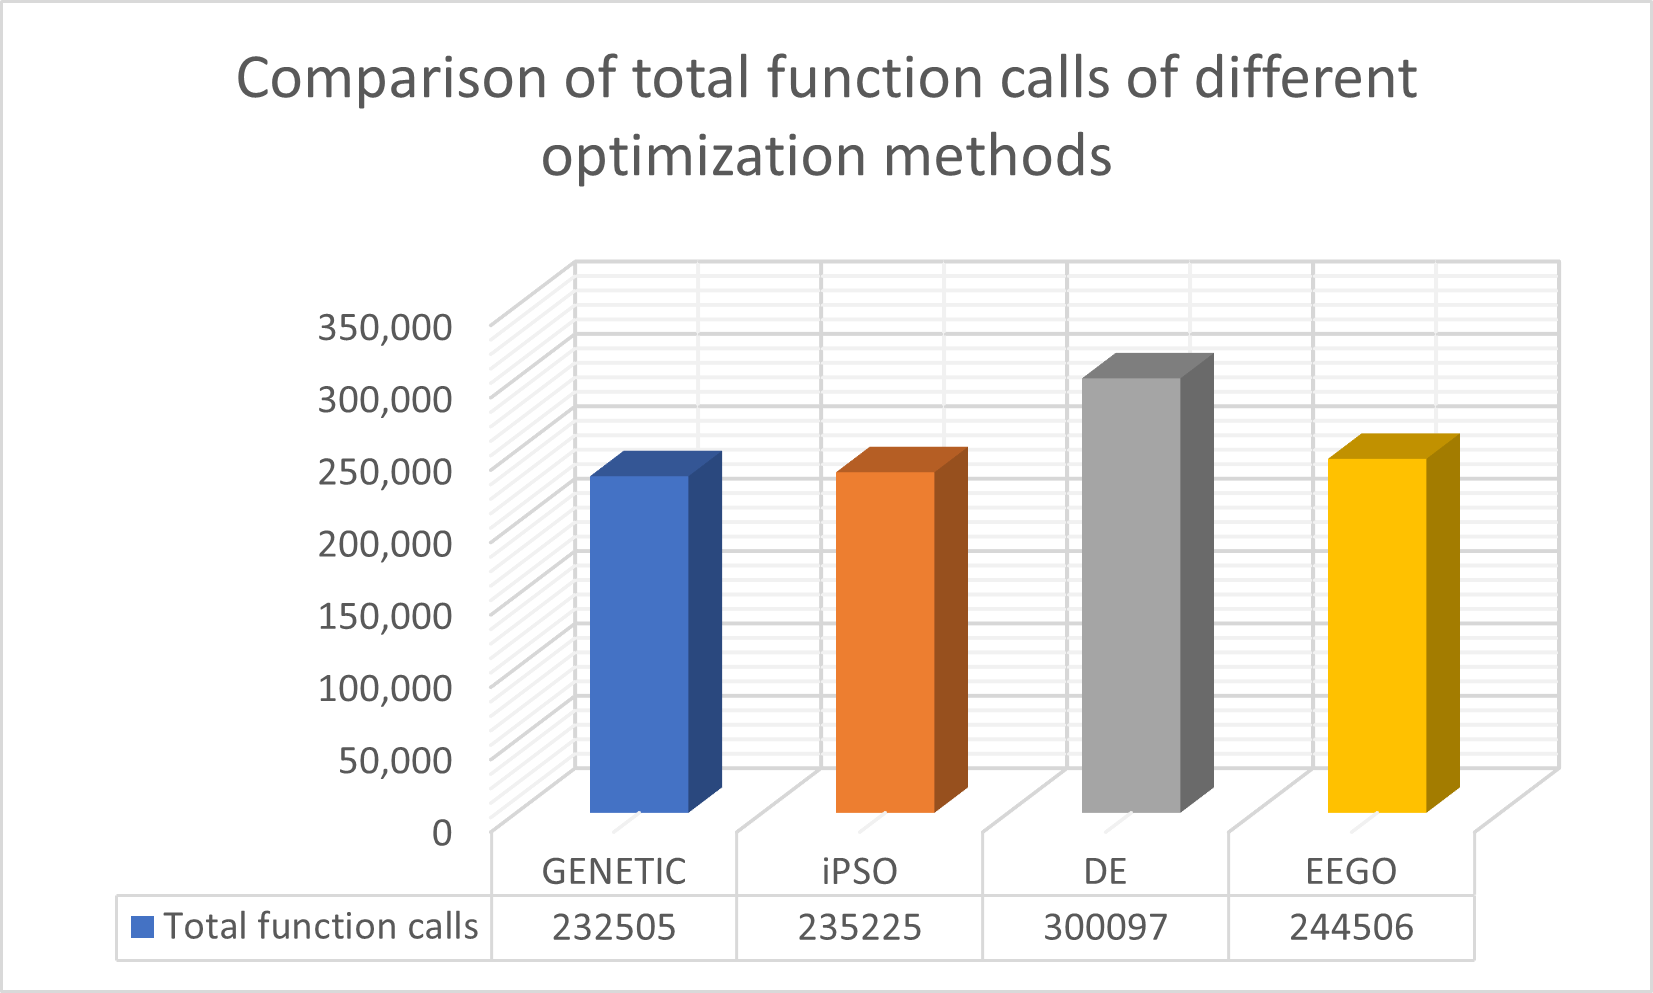
\includegraphics{image2}\caption{Total function calls for the different optimization methods, using
proposed initial distribution\label{fig:TotalFunctionCalls}}
\end{figure}
Also, a statistical comparison between the optimization methods is
shown graphically in Figure \ref{fig:functionCalls}.
\begin{figure}[H]
\centering{}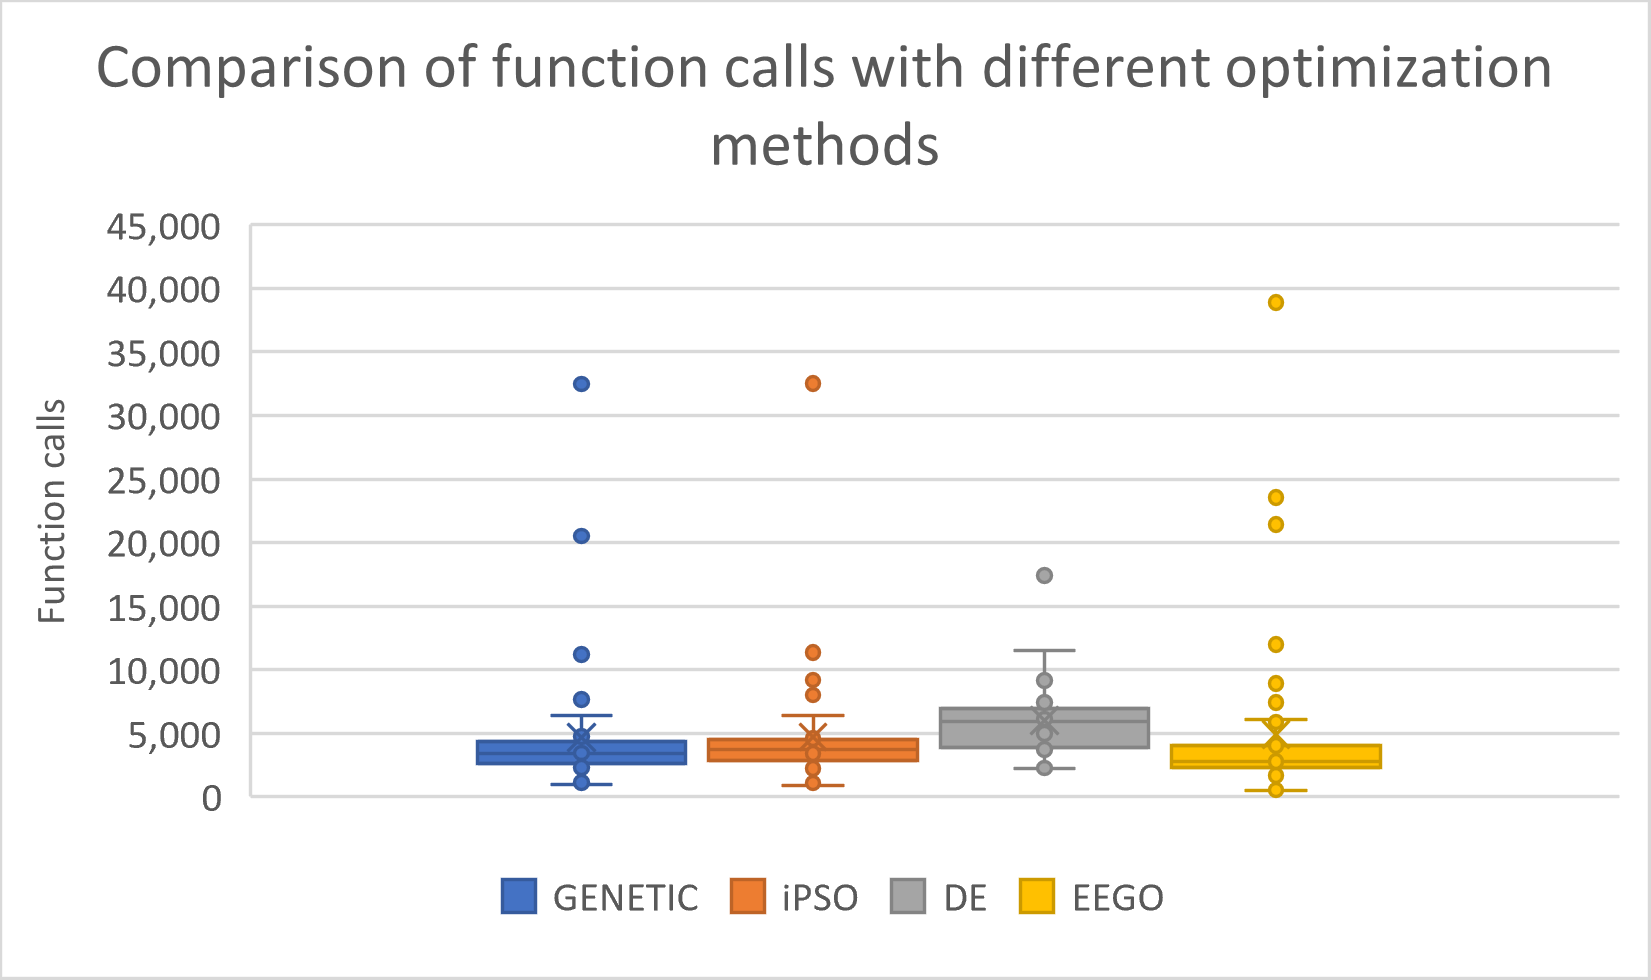
\includegraphics{image1}\caption{Comparison of function calls for the different optimization methods,
using proposed initial distribution\label{fig:functionCalls}}
\end{figure}

One more experiment which was performed with the ultimate goal of
measuring the importance of K-means sampling in the proposed method.
The results for this experiment are outlined in Table \ref{tab:sampling}
and the following sampling methods were used:
\begin{enumerate}
\item The column UNIFORM represents the application of uniform sampling
in the current method.
\item The column TRIANGULAR stands for the usage of the triangular distribution
\citep{triangular} for sampling.
\item The column MAXWELL stands for the application of the Maxwell distribution
\citep{maxwell} to produce initial samples for the used method.
\item The column KMEANS represents the usage of the method described in
subsection \ref{subsec:The-proposed-sampling} to produce initial
samples for the used method.
\end{enumerate}
\begin{table}[H]
\caption{Experiments using different sampling techniques for the proposed method.\label{tab:sampling}}

\centering{}%
\begin{tabular}{|c|c|c|c|c|}
\hline 
\textbf{FUNCTION} & \textbf{UNIFORM} & \textbf{TRIANGULAR} & \textbf{MAXWELL} & \textbf{KMEANS}\tabularnewline
\hline 
\hline 
BF1 & 4513 & 4318 & 4055 & 3228\tabularnewline
\hline 
BF2 & 3959 & 3879 & 3587 & 2815\tabularnewline
\hline 
BRANIN & 2282 & 2131 & 2066 & 1684\tabularnewline
\hline 
CAMEL & 3156 & 2919 & 2848 & 2262\tabularnewline
\hline 
EASOM & 1756 & 1650 & 1321 & 1334\tabularnewline
\hline 
EXP4 & 3438 & 3273 & 3194 & 2166\tabularnewline
\hline 
EXP8 & 3432 & 3387 & 3152 & 2802\tabularnewline
\hline 
EXP16 & 3369 & 3326 & 3291 & 3279\tabularnewline
\hline 
EXP32 & 3216 & 3225 & 3344 & 3430\tabularnewline
\hline 
GKLS250 & 2268 & 2023 & 1778 & 1603\tabularnewline
\hline 
GKLS350 & 2151 & 1841 & 2069 & 1298\tabularnewline
\hline 
GOLDSTEIN & 3855 & 3731 & 3530 & 2784\tabularnewline
\hline 
GRIEWANK2 & 4310 & 4510 & 4035 & 2589\tabularnewline
\hline 
GRIEWANK10 & 8640 & 8773 & 8232 & 7435\tabularnewline
\hline 
HANSEN & 3329 & 3071 & 2734 & 2484\tabularnewline
\hline 
HARTMAN3 & 2849 & 2673 & 2678 & 1793\tabularnewline
\hline 
HARTMAN6 & 3456 & 3249 & 3119 & 2478\tabularnewline
\hline 
POTENTIAL3 & 4554 & 5095 & 3928 & 4081\tabularnewline
\hline 
POTENTIAL5 & 8356 & 10032 & 7504 & 8886\tabularnewline
\hline 
RASTRIGIN & 3310 & 3187 & 2751 & 2304\tabularnewline
\hline 
ROSENBROCK4 & 6566 & 6353 & 5588 & 4019\tabularnewline
\hline 
ROSENBROCK8 & 8379 & 8717 & 7783 & 6801\tabularnewline
\hline 
ROSENBROCK16 & 11921 & 12471 & 11677 & 11996\tabularnewline
\hline 
SHEKEL5 & 3946 & 3731 & 3859 & 2495\tabularnewline
\hline 
SHEKEL7 & 3990 & 3646 & 3944 & 2432\tabularnewline
\hline 
SHEKEL10 & 3836 & 3630 & 3694 & 2516\tabularnewline
\hline 
TEST2N4 & 3345 & 3233 & 2867 & 2277\tabularnewline
\hline 
TEST2N5 & 3937 & 3742 & 3094 & 2734\tabularnewline
\hline 
TEST2N6 & 4008 & 4473 & 3266 & 2905\tabularnewline
\hline 
TEST2N7 & 4545 & 4612 & 3549 & 3559\tabularnewline
\hline 
SINU4 & 3128 & 2879 & 3559 & 2005\tabularnewline
\hline 
SINU8 & 4126 & 3767 & 5637 & 3158\tabularnewline
\hline 
SINU16 & 6774 & 5977 & 7739 & 5891\tabularnewline
\hline 
TEST30N3 & 3704 & 3384 & 3175 & 2362\tabularnewline
\hline 
TEST30N4 & 4262 & 4327 & 3491 & 2978\tabularnewline
\hline 
\textbf{SUM} & \textbf{152666} & \textbf{151235} & \textbf{142138} & \textbf{118863}\tabularnewline
\hline 
\end{tabular}
\end{table}

Initial distributions play a critical role in a wide range of applications,
including optimization, statistical analysis, and machine learning.
Table \ref{tab:sampling} presents the proposed distribution alongside
other established distributions. The uniform distribution is widely
used due to its ability to evenly cover the search space, making it
suitable for initializing optimization algorithms \citep{Browne}.
The triangular distribution is applied in scenarios where there is
knowledge of the bounds and the most probable value of a phenomenon,
making it useful in risk management models \citep{Zhao}. The Maxwell
distribution, although originating from physics, finds applications
in simulating communication networks, where data transfer speeds can
be modeled as random variables \citep{Chen}. Finally, the k-means
method is used for data clustering, with k-means++ initialization
offering improved performance compared to random distributions, particularly
in high-dimensional problems \citep{Xu}. As observed in Table \ref{tab:sampling},
the choice of an appropriate initial distribution can significantly
affect the performance of the algorithms that utilize them.

In the scatter plot in figure \ref{fig:ScatterPlot}, the critical
parameter \textquotedbl p\textquotedbl{} was found to be very small,
leading to the rejection of the null hypothesis and indicating that
the experimental results are highly significant.
\begin{figure}[H]
\centering{}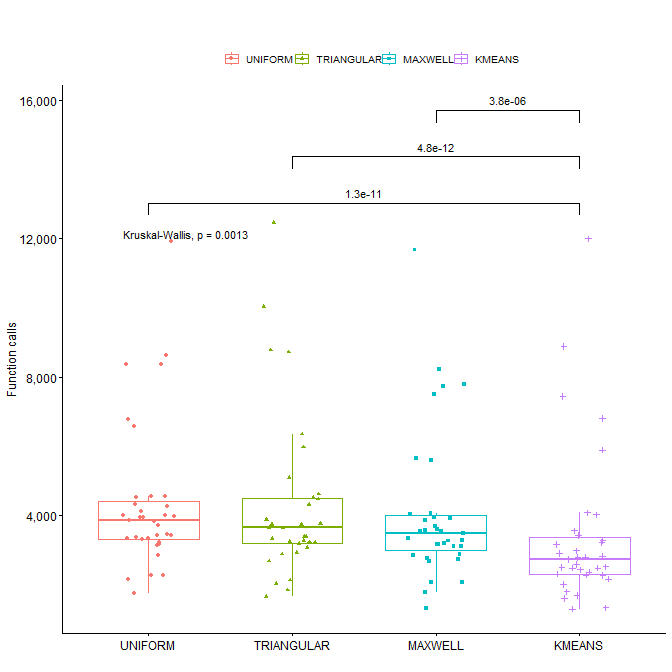
\includegraphics[scale=0.5]{image3}\caption{Scatter plot for different initial distributions\label{fig:ScatterPlot}}
\end{figure}
 

\section{Conclusions \label{sec:Conclusions}}

In the article, specific modifications to the EEGO optimization method
were proposed, which were mainly aimed at improving the efficiency
as well as the speed of the global optimization algorithm. The first
modification is the periodic application of a sampling technique based
on the K-Means method \citep{kmeans-ereunhtikh-koinothta}. Using
the sampling method we proposed helped to find the global minimum
with the greatest accuracy and in the least possible time. The above
procedure significantly reduced the required number of function calls
compared to other random distributions, even in difficult multidimensional
functions. The second proposed modification concerns the similarity
termination rule, which helps avoid wasting unnecessary computing
time on iterations. In addition, we proposed some modifications which
significantly help to reduce the number of calls and increase the
success rate of the algorithm. Because the experimental results are
promising, efforts can be made to develop the technique in various
areas. A future extension of the implementation may be the use of
parallel computing techniques to speed up the optimization process,
such as, for example, the integration of MPI \citep{MPI} or the OpenMP
library \citep{OPENMP}.

\vspace{6pt}


\authorcontributions{G.K., V.C. and I.G.T. conceived of the idea and the methodology,
and G.K. and V.C. implemented the corresponding software. G.K. conducted
the experiments, employing objective functions as test cases, and
provided the comparative experiments. I.G.T. performed the necessary
statistical tests. All authors have read and agreed to the published
version of the manuscript.}

\funding{This research received no external funding.}

\institutionalreview{Not applicable.}

\informedconsent{Not applicable.}

\dataavailability{The original contributions presented in the study are included in
the article, further inquiries can be directed to the corresponding
author.}

\acknowledgments{This research has been financed by the European Union: Next Generation
EU through the Program Greece 2.0 National Recovery and Resilience
Plan, under the call RESEARCH--CREATE--INNOVATE, project name “iCREW:
Intelligent small craft simulator for advanced crew training using
Virtual Reality techniques” (project code: TAEDK-06195).}

\conflictsofinterest{The authors declare no conflicts of interest.}

\appendixtitles{no}

\appendixstart{}

\appendix

\begin{adjustwidth}{-\extralength}{0cm}{}

\reftitle{References}
\begin{thebibliography}{999}
\bibitem{plhroforikh}A. Törn, M.M. Ali, S. Viitanen, Stochastic global
optimization: Problem classes and solution techniques. Journal of
Global Optimization \textbf{14}, pp. 437-447, 1999.

\bibitem{computer}Floudas, C. A., \& Pardalos, P. M. (Eds.). (2013).
State of the art in global optimization: computational methods and
applications

\bibitem{computer1}Horst, R., \& Pardalos, P. M. (Eds.). (2013).
Handbook of global optimization (Vol. 2). Springer Science \& Business
Media.

\bibitem{maths}Intriligator, M. D. (2002). Mathematical optimization
and economic theory. Society for Industrial and Applied Mathematics.

\bibitem{maths-1}Cánovas, M. J., Kruger, A., Phu, H. X., \& Théra,
M. (2020). Marco A. López, a Pioneer of Continuous Optimization in
Spain. Vietnam Journal of Mathematics, 48, 211-219.

\bibitem{maths2}Mahmoodabadi, M. J., \& Nemati, A. R. (2016). A novel
adaptive genetic algorithm for global optimization of mathematical
test functions and real-world problems. Engineering Science and Technology,
an International Journal, 19(4), 2002-2021.

\bibitem{key-maths3}Li, J., Xiao, X., Boukouvala, F., Floudas, C.
A., Zhao, B., Du, G., ... \& Liu, H. (2016). Data‐driven mathematical
modeling and global optimization framework for entire petrochemical
planning operations. AIChE Journal, 62(9), 3020-3040.

\bibitem{fusikh}E. Iuliano, Global optimization of benchmark aerodynamic
cases using physics-based surrogate models, Aerospace Science and
Technology \textbf{67}, pp.273-286, 2017.

\bibitem{fusikh1}Q. Duan, S. Sorooshian, V. Gupta, Effective and
efficient global optimization for conceptual rainfall-runoff models,
Water Resources Research \textbf{28}, pp. 1015-1031 , 1992.

\bibitem{fysikhh}L. Yang, D. Robin, F. Sannibale, C. Steier, W. Wan,
Global optimization of an accelerator lattice using multiobjective
genetic algorithms, Nuclear Instruments and Methods in Physics Research
Section A: Accelerators, Spectrometers, Detectors and Associated Equipment
\textbf{609}, pp. 50-57, 2009.

\bibitem{xhmeia}S. Heiles, R. L. Johnston, Global optimization of
clusters using electronic structure methods, Int. J. Quantum Chem.
\textbf{113}, pp. 2091-- 2109, 2013.

\bibitem{xhmeia1}W.H. Shin, J.K. Kim, D.S. Kim, C. Seok, GalaxyDock2:
Protein--ligand docking using beta-complex and global optimization,
J. Comput. Chem. \textbf{34}, pp. 2647-- 2656, 2013.

\bibitem{xhmeia2}A. Liwo, J. Lee, D.R. Ripoll, J. Pillardy, H. A.
Scheraga, Protein structure prediction by global optimization of a
potential energy function, Biophysics \textbf{96}, pp. 5482-5485,
1999.

\bibitem{iatrikh}Eva K. Lee, Large-Scale Optimization-Based Classification
Models in Medicine and Biology, Annals of Biomedical Engineering \textbf{35},
pp 1095-1109, 2007.

\bibitem{iatrikh1}Y. Cherruault, Global optimization in biology and
medicine, Mathematical and Computer Modelling \textbf{20}, pp. 119-132,
1994.

\bibitem{medicine}Houssein, E. H., Hosney, M. E., Mohamed, W. M.,
Ali, A. A., \& Younis, E. M. (2023). Fuzzy-based hunger games search
algorithm for global optimization and feature selection using medical
data. Neural Computing and Applications, 35(7), 5251-5275.

\bibitem{determistic}Ion, I. G., Bontinck, Z., Loukrezis, D., Römer,
U., Lass, O., Ulbrich, S., ... \& De Gersem, H. (2018). Robust shape
optimization of electric devices based on deterministic optimization
methods and finite-element analysis with affine parametrization and
design elements. Electrical Engineering, 100(4), 2635-2647.

\bibitem{determistic1}Cuevas-Velásquez, V., Sordo-Ward, A., García-Palacios,
J. H., Bianucci, P., \& Garrote, L. (2020). Probabilistic model for
real-time flood operation of a dam based on a deterministic optimization
model. Water, 12(11), 3206.

\bibitem{determistic2}Pereyra, M., Schniter, P., Chouzenoux, E.,
Pesquet, J. C., Tourneret, J. Y., Hero, A. O., \& McLaughlin, S. (2015).
A survey of stochastic simulation and optimization methods in signal
processing. IEEE Journal of Selected Topics in Signal Processing,
10(2), 224-241.

\bibitem{stohastic}Hannah, L. A. (2015). Stochastic optimization.
International Encyclopedia of the Social \& Behavioral Sciences, 2,
473-481.

\bibitem{stohastic1}Kizielewicz, B., \& Sałabun, W. (2020). A new
approach to identifying a multi-criteria decision model based on stochastic
optimization techniques. Symmetry, 12(9), 1551.

\bibitem{stohastic2}Chen, T., Sun, Y., \& Yin, W. (2021). Solving
stochastic compositional optimization is nearly as easy as solving
stochastic optimization. IEEE Transactions on Signal Processing, 69,
4937-4948.

\bibitem{key-1}M.A. Wolfe, Interval methods for global optimization,
Applied Mathematics and Computation \textbf{75}, pp. 179-206, 1996.

\bibitem{interval2}T. Csendes and D. Ratz, Subdivision Direction
Selection in Interval Methods for Global Optimization, SIAM J. Numer.
Anal. \textbf{34}, pp. 922--938, 1997. 

\bibitem{swarm1}Hassanien, A. E., \& Emary, E. (2018). Swarm intelligence:
principles, advances, and applications. CRC press.

\bibitem{swarm2}Tang, J., Liu, G., \& Pan, Q. (2021). A review on
representative swarm intelligence algorithms for solving optimization
problems: Applications and trends. IEEE/CAA Journal of Automatica
Sinica, 8(10), 1627-1643.

\bibitem{swarm}Brezočnik, L., Fister Jr, I., \& Podgorelec, V. (2018).
Swarm intelligence algorithms for feature selection: a review. Applied
Sciences, 8(9), 1521.

\bibitem{APPS}Tang, J., Liu, G., Pan, Q.: A review on representative
swarm intelligence algorithms for solving optimization problems:applications
and trends. IEEE/CAA J. Autom. Sin. 8(10),1627--1643 (2021)

\bibitem{WOA}Mirjalili, S., Lewis, A.: The whale optimization algorithm.
Adv. Eng. Softw. 95, 51--67 (2016)

\bibitem{WOA1}Nasiri, J., \& Khiyabani, F. M. (2018). A whale optimization
algorithm (WOA) approach for clustering. Cogent Mathematics \& Statistics,
5(1), 1483565.

\bibitem{WOA2}Gharehchopogh, F. S., \& Gholizadeh, H. (2019). A comprehensive
survey: Whale Optimization Algorithm and its applications. Swarm and
Evolutionary Computation, 48, 1-24.

\bibitem{SCA}Mirjalili, S.: SCA: a sine cosine algorithm for solving
optimization problems. Knowl.-Based Syst. 96, 120--133 (2016)

\bibitem{SCA1}Hao, Y., Song, L., Cui, L., \& Wang, H. (2019). A three-dimensional
geometric features-based SCA algorithm for compound faults diagnosis.
Measurement, 134, 480-491.

\bibitem{SCA2}Sahu, P. C., Prusty, R. C., \& Panda, S. (2022). Optimal
design of a robust FO-Multistage controller for the frequency awareness
of an islanded AC microgrid under i-SCA algorithm. International Journal
of Ambient Energy, 43(1), 2681-2693.

\bibitem{sca1}Zivkovic, M., Stoean, C., Chhabra, A., Budimirovic,
N., Petrovic, A., \& Bacanin, N. (2022). Novel improved salp swarm
algorithm: An application for feature selection. Sensors, 22(5), 1711.

\bibitem{ssaa}Wan, Y., Mao, M., Zhou, L., Zhang, Q., Xi, X., \& Zheng,
C. (2019). A novel nature-inspired maximum power point tracking (MPPT)
controller based on SSA-GWO algorithm for partially shaded photovoltaic
systems. Electronics, 8(6), 680.

\bibitem{SSA}Mirjalili, S., Gandomi, A.H., Mirjalili, S.Z., Saremi,
S., Faris, H., Mirjalili, S.M.: Salp swarm algorithm: a bio-inspired
optimizer for engineering design problems. Adv. Eng. Softw. 114, 163--191
(2017)

\bibitem{SSA1}Bairathi, D., \& Gopalani, D. (2019). Salp swarm algorithm
(SSA) for training feed-forward neural networks. In Soft Computing
for Problem Solving: SocProS 2017, Volume 1 (pp. 521-534). Springer
Singapore.

\bibitem{SSA2}Abualigah, L., Shehab, M., Alshinwan, M., \& Alabool,
H. (2020). Salp swarm algorithm: a comprehensive survey. Neural Computing
and Applications, 32(15), 11195-11215.

\bibitem{search algorithm} Usman, M.J.: A survey of symbiotic organisms
search algorithms and applications. Neural Comput. Appl. 32(2), 547--566
(2020)

\bibitem{several metaheuristic algorithms }. Ezugwu, A.E., Adeleke,
O.J., Akinyelu, A.A., Viriri, S.: A conceptual comparison of several
metaheuristic algorithms on continuous optimisation problems. Neural
Comput. Appl. 32(10), 6207--6251 (2020)

\bibitem{mutualism-parasitism}Wang, Y., \& DeAngelis, D. L. (2012).
A mutualism-parasitism system modeling host and parasite withmutualism
at low density. Mathematical Biosciences \& Engineering, 9(2), 431-444.

\bibitem{mutualistic}Aubier, T. G., Joron, M., \& Sherratt, T. N.
(2017). Mimicry among unequally defended prey should be mutualistic
when predators sample optimally. The American Naturalist, 189(3),
267-282.

\bibitem{Competition in mutualistic systems}Addicott, J. F. (1985).
Competition in mutualistic systems. The biology of mutualism: ecology
and evolution. Croom Helm, London, UK, 217-247.

\bibitem{hunting between groupers and giant moray eels in the Red Sea}Bshary,
R., Hohner, A., Ait-el-Djoudi, K., Fricke, H.: Interspecific communicative
and coordinated hunting between groupers and giant moray eels in the
Red Sea. PLoS Biol. 4(12), e431 (2006)

\bibitem{Eel and grouper optimizer}Ali Mohammadzadeh, Seyedali Mirjalili.
(2024) Eel and grouper optimizer: a nature-inspired optimization algorithm.
Springer Science+Business Media, LLC, part of Springer Nature 2024

\bibitem{kmeans2}P. Arora, S. Varshney, Analysis of k-means and k-medoids
algorithm for big data, Procedia Computer Science \textbf{78}, pp.
507-512, 2016.

\bibitem{kmeans-ereunhtikh-koinothta}Ahmed, M., Seraj, R., \& Islam,
S. M. S. (2020). The k-means algorithm: A comprehensive survey and
performance evaluation. Electronics, 9(8), 1295.

\bibitem{charilogis}Charilogis, V.; Tsoulos, I.G. Toward an Ideal
Particle Swarm Optimizer for Multidimensional Functions. Information
2022, 13, 217. 

\bibitem{MacQueen}J.B. MacQueen, Some Methods for classification
and Analysis of Multivariate Observations. Proceedings of 5th Berkeley
Symposium on Mathematical Statistics and Probability. Vol. 1. University
of California Press. pp. 281--297. MR 0214227. Zbl 0214.46201, 1967.

\bibitem{kmeans1-1}Y. Li, H. Wu, A clustering method based on K-means
algorithm, Physics Procedia \textbf{25}, pp. 1104-1109, 2012.

\bibitem{kmeans-paterrn}Ali, H. H., \& Kadhum, L. E. (2017). K-means
clustering algorithm applications in data mining and pattern recognition.
International Journal of Science and Research (IJSR), 6(8), 1577-1584.

\bibitem{Ali}M. Montaz Ali, Charoenchai Khompatraporn, Zelda B. Zabinsky,
A Numerical Evaluation of Several Stochastic Algorithms on Selected
Continuous Global Optimization Test Problems, Journal of Global Optimization
\textbf{31}, pp 635-672, 2005. 

\bibitem{Floudas1}C.A. Floudas, P.M. Pardalos, C. Adjiman, W. Esposoto,
Z. G$\ddot{\mbox{u}}$m$\ddot{\mbox{u}}$s, S. Harding, J. Klepeis,
C. Meyer, C. Schweiger, Handbook of Test Problems in Local and Global
Optimization, Kluwer Academic Publishers, Dordrecht, 1999.

\bibitem{testfunc1}M.M. Ali and P. Kaelo, Improved particle swarm
algorithms for global optimization, Applied Mathematics and Computation
\textbf{196}, pp. 578-593, 2008.

\bibitem{testfunc2}H. Koyuncu, R. Ceylan, A PSO based approach: Scout
particle swarm algorithm for continuous global optimization problems,
Journal of Computational Design and Engineering \textbf{6}, pp. 129--142,
2019.

\bibitem{testfunc2-1}Patrick Siarry, Gérard Berthiau, François Durdin,
Jacques Haussy, ACM Transactions on Mathematical Software \textbf{23},
pp 209--228, 1997.

\bibitem{testfunc3}I.G. Tsoulos, I.E. Lagaris, GenMin: An enhanced
genetic algorithm for global optimization, Computer Physics Communications\textbf{
178, }pp. 843-851, 2008.

\bibitem{testfunc4}A. LaTorre, D. Molina, E. Osaba, J. Poyatos, J.
Del Ser, F. Herrera, A prescription of methodological guidelines for
comparing bio-inspired optimization algorithms, Swarm and Evolutionary
Computation \textbf{67}, 100973, 2021.

\bibitem{gkls}M. Gaviano, D.E. Ksasov, D. Lera, Y.D. Sergeyev, Software
for generation of classes of test functions with known local and global
minima for global optimization, ACM Trans. Math. Softw. \textbf{29},
pp. 469-480, 2003.

\bibitem{jones}J.E. Lennard-Jones, On the Determination of Molecular
Fields, Proc. R. Soc. Lond. A \textbf{ 106}, pp. 463--477, 1924.

\bibitem{powell}Powell, M.J.D. A Tolerant Algorithm for Linearly
Constrained Optimization Calculations. Math. Program. 1989, 45, 547--566.

\bibitem{genetic1}D. Goldberg, Genetic Algorithms in Search, Optimization
and Machine Learning, Addison-Wesley Publishing Company, Reading,
Massachussets, 1989.

\bibitem{genetic2}Z. Michaelewicz, Genetic Algorithms + Data Structures
= Evolution Programs. Springer - Verlag, Berlin, 1996.

\bibitem{doublepop}I.G. Tsoulos, Modifications of real code genetic
algorithm for global optimization, Applied Mathematics and Computation
203, pp. 598-607, 2008.

\bibitem{pso1}Riccardo Poli, James Kennedy kennedy, Tim Blackwell,
Particle swarm optimization An Overview, Swarm Intelligence \textbf{1},
pp 33-57, 2007. 

\bibitem{pso2}Ioan Cristian Trelea, The particle swarm optimization
algorithm: convergence analysis and parameter selection, Information
Processing Letters \textbf{85}, pp. 317-325, 2003.

\bibitem{ipso}V. Charilogis, I.G. Tsoulos, Toward an Ideal Particle
Swarm Optimizer for Multidimensional Functions , Information \textbf{13},
217, 2022.

\bibitem{diffe1}R. Storn, K. Price, Differential Evolution - A Simple
and Efficient Heuristic for Global Optimization over Continuous Spaces,
Journal of Global Optimization \textbf{11}, pp. 341-359, 1997.

\bibitem{diffe2}J. Liu, J. Lampinen, A Fuzzy Adaptive Differential
Evolution Algorithm. Soft Comput \textbf{9}, pp.448--462, 2005.

\bibitem{gao}Alsayyed, O.; Hamadneh, T.; Al-Tarawneh, H.; Alqudah,
M.; Gochhait, S.; Leonova, I.; Malik, O.P.; Dehghani, M. Giant Armadillo
Optimization: A New Bio-Inspired Metaheuristic Algorithm for Solving
Optimization Problems. Biomimetics 2023, 8, 619.

\bibitem{igao}Kyrou G, Charilogis V, Tsoulos IG. Improving the Giant-Armadillo
Optimization Method. Analytics. 2024; 3(2):225-240. https://doi.org/10.3390/analytics3020013 

\bibitem{triangular}W.E. Stein, M.F. Keblis, A new method to simulate
the triangular distribution, Mathematical and Computer Modelling Volume
\textbf{49}, pp. 1143-1147, 2009.

\bibitem{maxwell}Sharma, V. K., Bakouch, H. S., \& Suthar, K. (2017).
An extended Maxwell distribution: Properties and applications. Communications
in Statistics-Simulation and Computation, 46(9), 6982-7007.

\bibitem[(2022)]{Browne}Browne, D. et al., (2022). Applications of
Uniform Distributions in Optimization Algorithms. Journal of Applied
Statistics, 45(2), 123-139.

\bibitem[(2023)]{Zhao}Zhao, Y., et al., (2023). Risk Management Models
Using Triangular Distributions. Risk Analysis Quarterly, 39(1), 98-112.

\bibitem[(2021)]{Chen}Chen, L., et al., (2021). Simulating Communication
Networks with Maxwell Distribution. IEEE Transactions on Communications,
68(4), 568-578.

\bibitem[(2022)]{Xu}Xu, J., et al., (2022). Improving K-means Clustering
with K-means++ Initialization. Machine Learning Journal, 34(3), 245-267.

\bibitem{MPI}Gropp, W.; Lusk, E.; Doss, N.; Skjellum, A. A high-performance,
portable implementation of the MPI message passing interface standard.
Parallel Comput. 1996, 22, 789--828. 

\bibitem{OPENMP}Chandra, R. Parallel Programming in OpenMP; Morgan
Kaufmann: Cambridge, MA, USA, 2001.

\bibitem{scaa}Gad, A. G. (2022). Particle swarm optimization algorithm
and its applications: a systematic review. Archives of computational
methods in engineering, 29(5), 2531-2561.

\end{thebibliography}
%%%%%%%%%%%%%%%%%%%%%%%%%%%%%%%%%%%%%%%%%%
%% for journal Sci
%\reviewreports{\\
%Reviewer 1 comments and authors' response\\
%Reviewer 2 comments and authors' response\\
%Reviewer 3 comments and authors' response
%}
%%%%%%%%%%%%%%%%%%%%%%%%%%%%%%%%%%%%%%%%%%

\PublishersNote{}

\end{adjustwidth}{}
\end{document}
